El proyecto sTGC Minería se compone de tres sistemas principales: disparo, detección y adquisición, como se ilustra en la Figura \ref{fig:sistema-completo}. Como se introdujo en la Sección \ref{sec:planteamiento}, el sistema de disparo \cite{Oyanadel2020SistemaSTGC} (ilustrado en morado) ya ha sido construido en el CCTVal y está formado por dos detectores centelladores y una unidad de coincidencias que emite una señal digital de disparo (indicada en morado) cuando un muon traspasa ambos detectores centelladores. Esta señal de disparo es necesaria para discriminar eventos captados por el detector sTGC y descartar interacciones procedentes de otras partículas cargadas que no sean muones.
	
Si bien los detectores centelladores presentes en el sistema de disparo son capaces de detectar exclusivamente el paso de muones, estos no son capaces de determinar la ubicación del vértice de interacción y solo se utilizan como detectores complementarios. Para localizar vértices de interacción se utiliza el sistema de detección sTGC fabricado por CCTVal (ilustrado en verde en la Figura \ref{fig:sistema-completo}), que gracias a su tecnología de fabricación permite determinar la ubicación de los vértices con resoluciones de 1cm$^2$ o incluso mejores.
	
En este capítulo se detalla la forma y funcionamiento del sistema de detección, describiendo el prototipo de detector sTGC utilizado en sTGC Minería y describiendo también la interfaz de lectura ASD. Este sistema de detección ya ha sido construido y probado por CCTVal, pero es necesario conocer sus características para entender su funcionamiento, así como también para determinar la cantidad y tipos de señales a leer en el sistema de adquisición de datos que se diseñará en esta memoria de titulación.
	
	\begin{figure}[h]
		\centering
		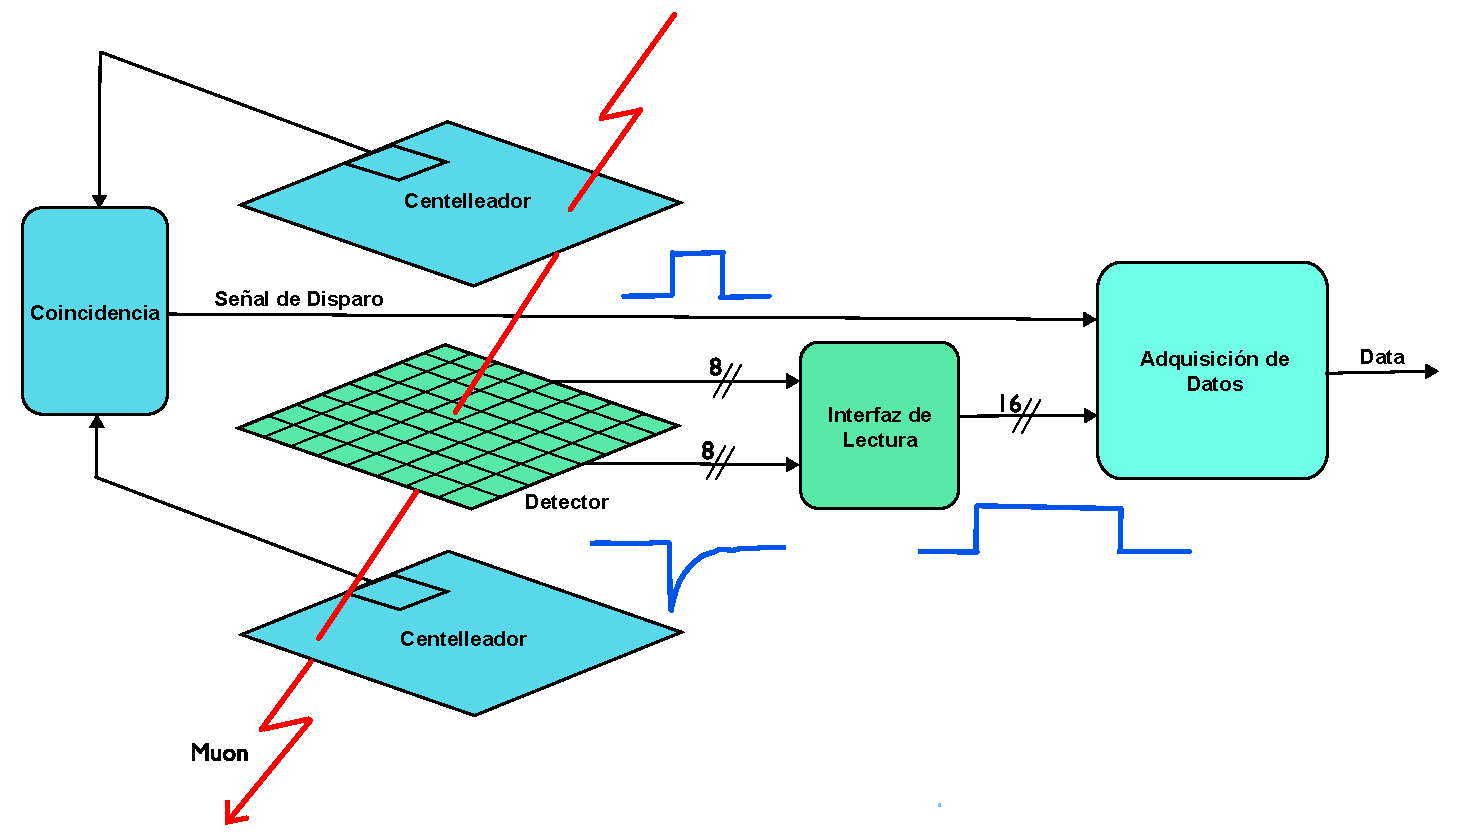
\includegraphics[scale=0.55]{sistema.pdf}
		\caption{Diagrama del sistema de muongrafía de terreno utilizando un solo detector.}
		\label{fig:sistema-completo}
	\end{figure}